\documentclass{beamer}
\usetheme{Madrid}

\title{Cheap calibration of the normalizing flow using arbitrary classifier}
\author{by Robert Drynkin, Maxim Artemev, Denis Derkach}
\centering
\date{April 2020}
\begin{document}
\maketitle

\begin{frame}{Content}
  \begin{itemize}
    \item Assumptions
    \item Idea
    \item Implemetation details
    \item Pictures
    \item Current results
    \item FAQ
  \end{itemize}
\end{frame}

\begin{frame}{Assumptions}
  
  \begin{columns}[T] % align columns
    \begin{column}{.48\textwidth}

      Normalizing flows
      \begin{itemize}
        \item - Long time to train
        \item - Unstable training
        \item - Have an artefacts due to continuity
        \item + Generative model
      \end{itemize}
    \end{column}%
  \hfill%
  \begin{column}{.48\textwidth}
  
    Binary classifier
    \begin{itemize}
      \item + Fast training
      \item + A lot of libraries
      \item + Well studied
      \item - Not a generative model
    \end{itemize}
  \end{column}%
  \end{columns}

  Can we use binary classifier to improve normalizing flow with the preservation of useful properties?

\end{frame}

\begin{frame}{Idea}
  $Q(x)$ -- density of the real distribution\\
  $P(x)$ -- density of the distribution given by nf\\
  $clf(x)$ -- prediction of the perfect discriminator (binary classifier which trained to distinguish samples from Q and P) \newline

  We can express $Q(x)$ using only $P(x)$ and $clf(x)$
  $$ clf - \text{perfect} \Rightarrow clf(x) = \frac{Q(x)}{P(x) + Q(x)} \Rightarrow \frac{clf(x)}{1 - clf(x)} = \frac{Q(x)}{P(x)} $$
  $$ Q(x) = P(x) \frac{clf(x)}{1 - clf(x)} $$

\end{frame}

\begin{frame}{Implemetation details}
  For the numerical stability:
  $$ \log Q(x) = \log P(x) + clf\_logit(x) $$
  Sampling: rejection sampling from $Q(x)$ using $c \cdot P(x)$ as a major distribution.
  Acceptance rate equals to $1/c$, where $c = \max \exp clf\_logit(x) $
\end{frame}

\begin{frame}{Pictures}
  \begin{columns}[T] % align columns
    \begin{column}{.48\textwidth}
      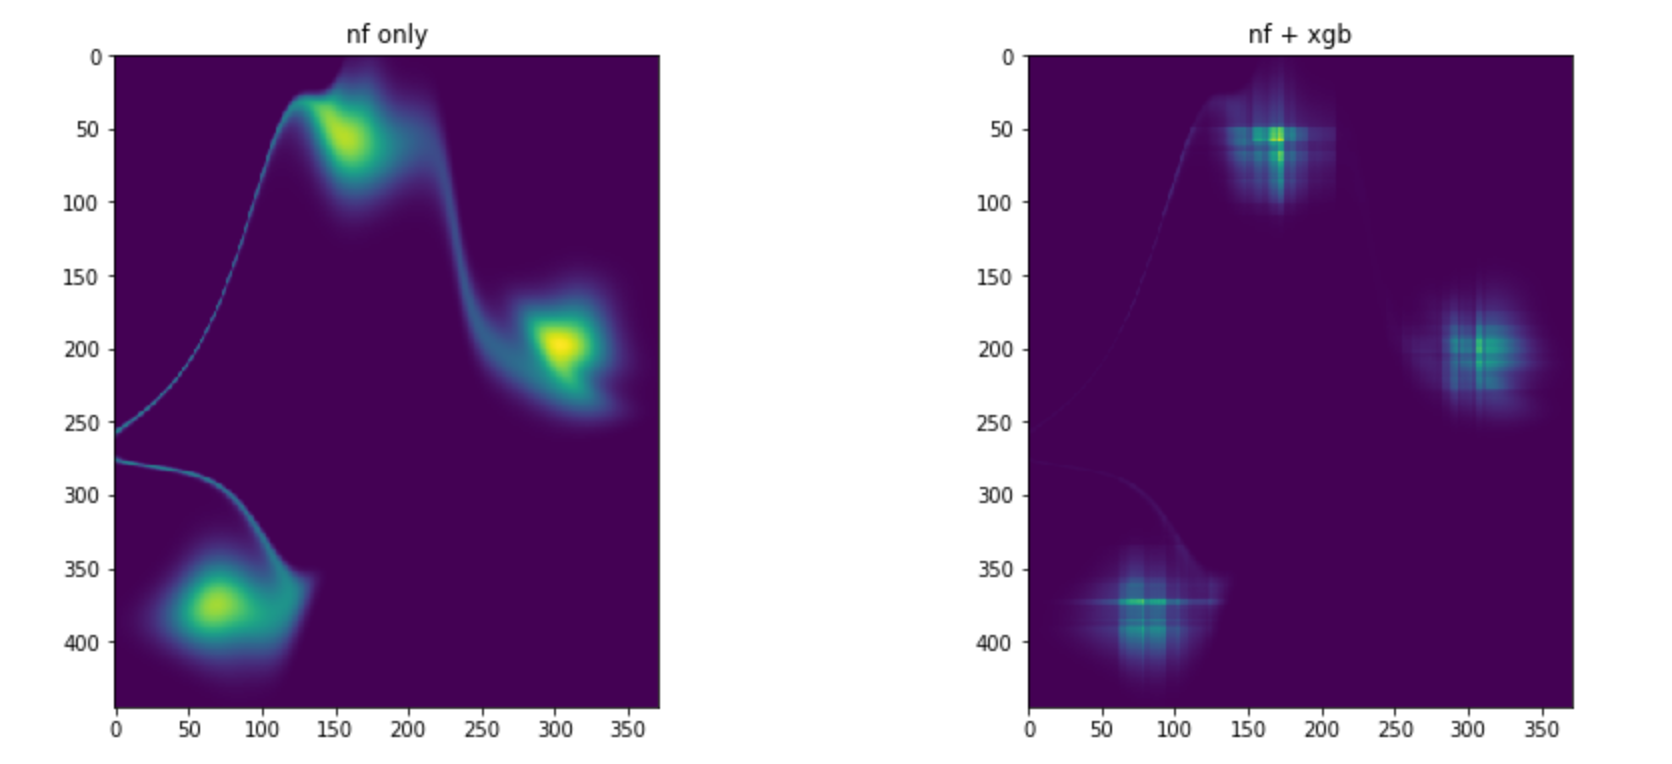
\includegraphics[width=5.5cm]{imgs/blob_dens.png}
      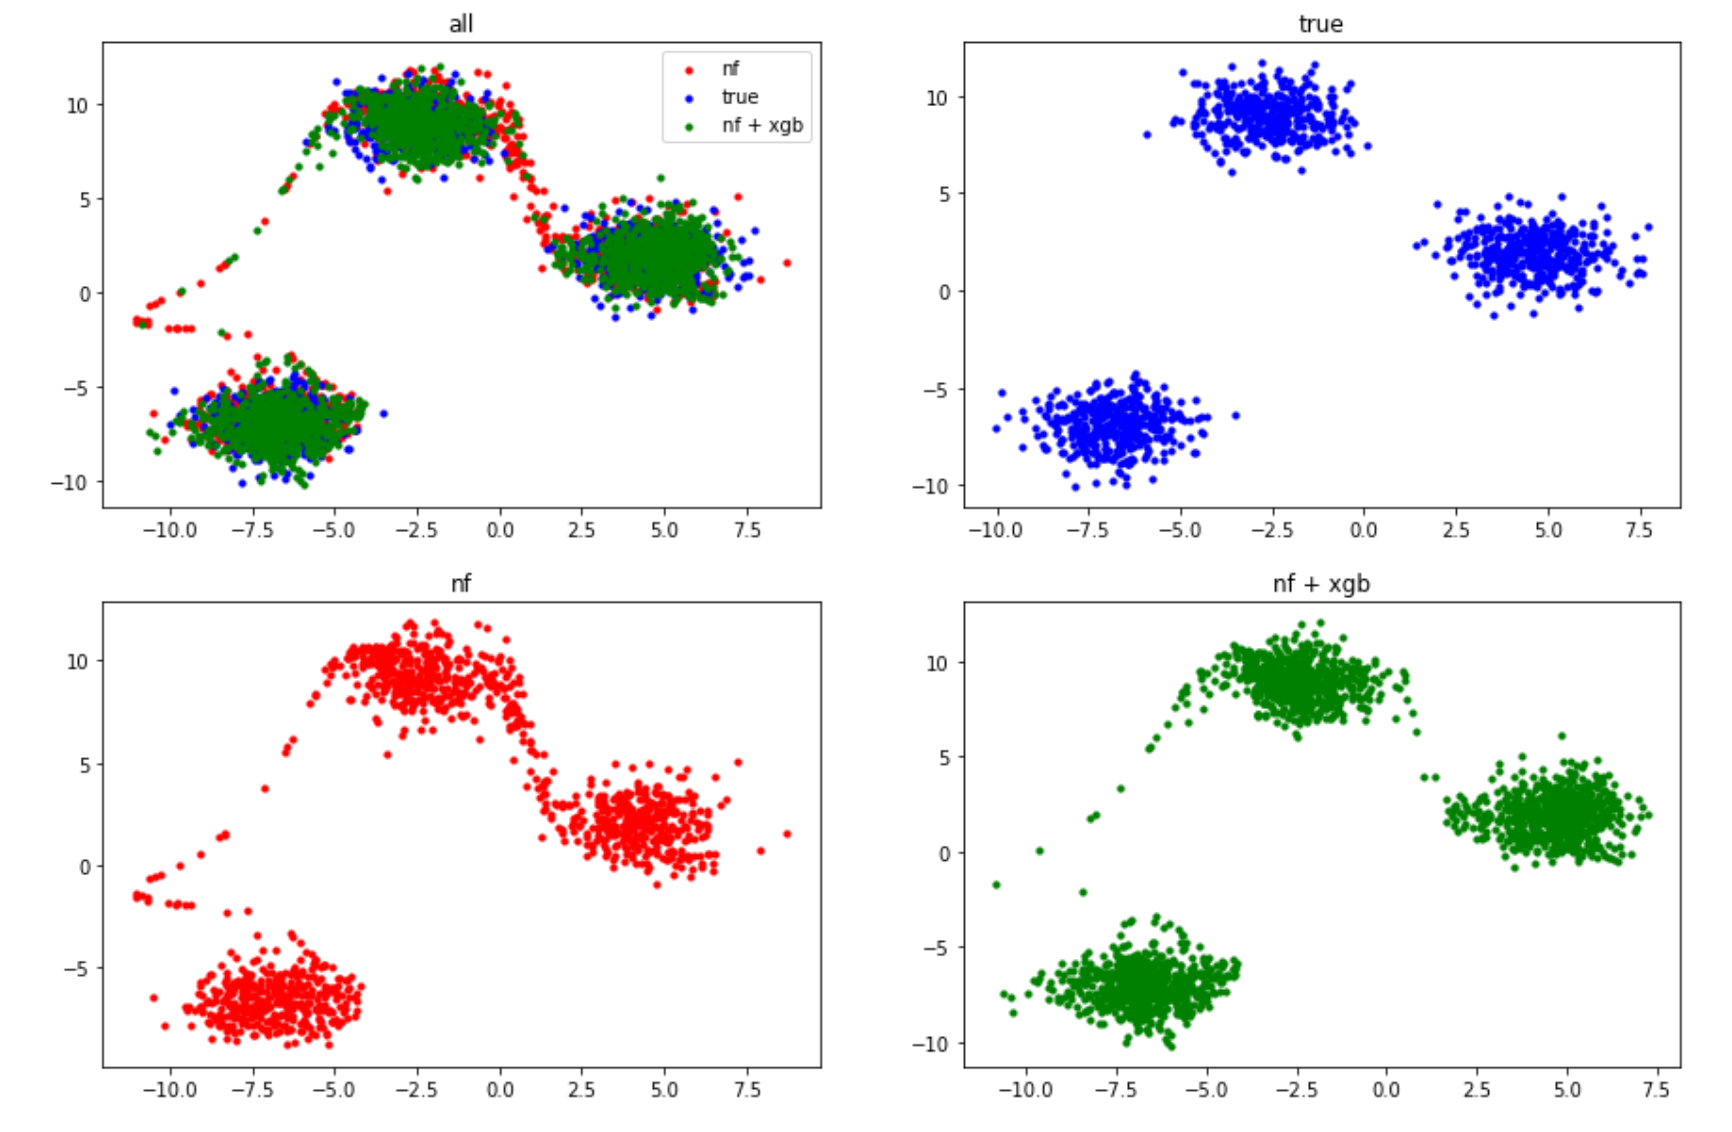
\includegraphics[width=5.5cm]{imgs/blob_sample.png}
    \end{column}%
    \hfill%
    \begin{column}{.48\textwidth}
      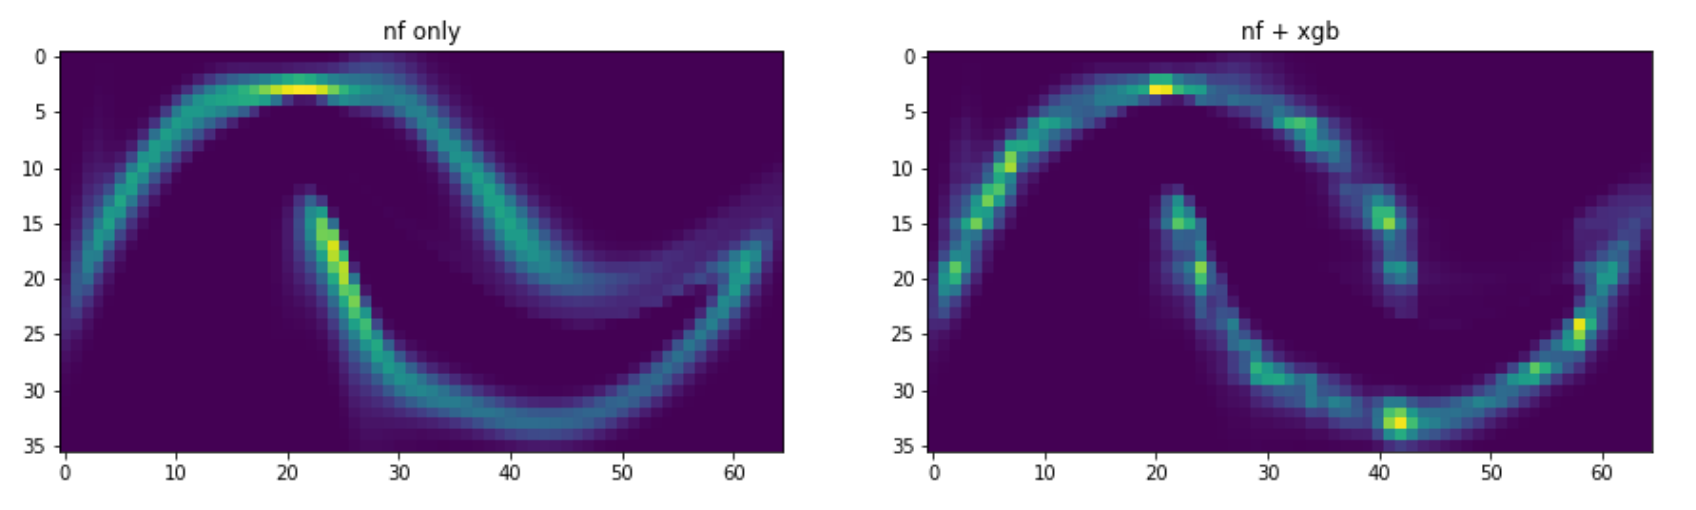
\includegraphics[width=5.5cm]{imgs/moons_dens.png}
      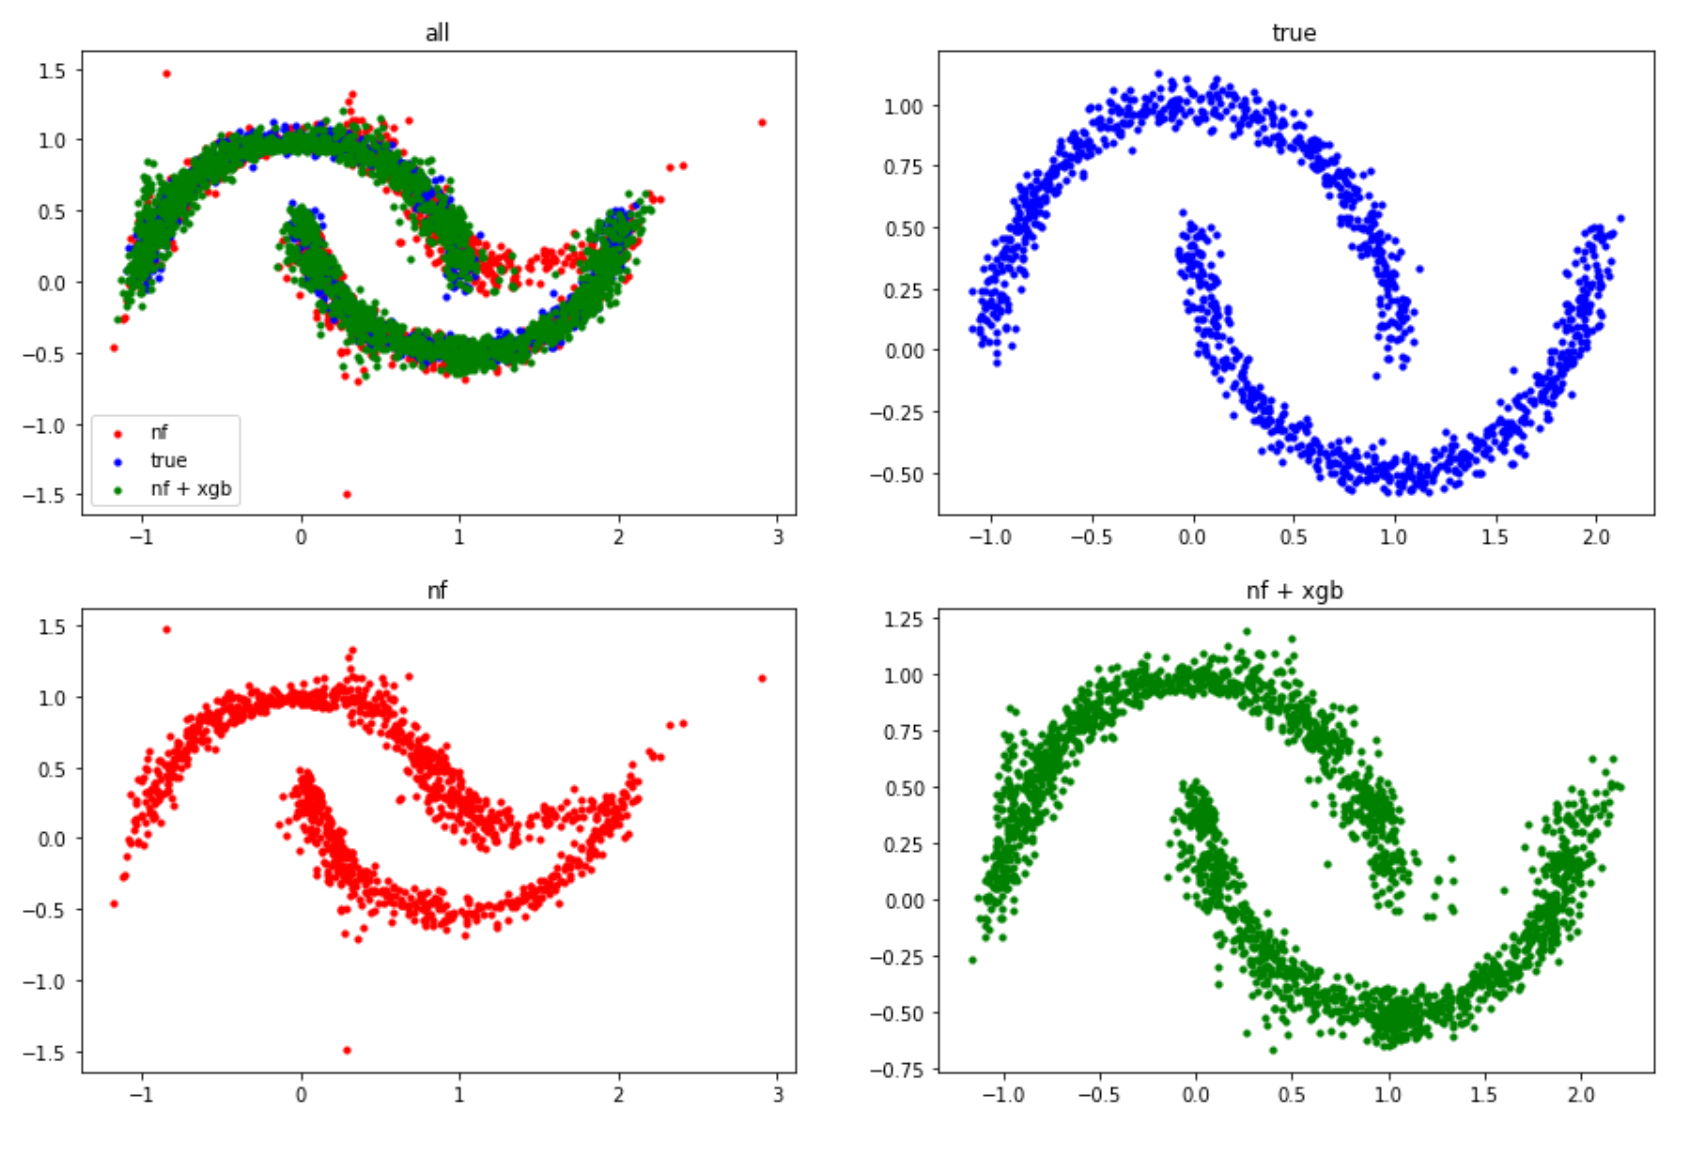
\includegraphics[width=5.5cm]{imgs/moons_sample.png}
    \end{column}%
  \end{columns}
\end{frame}

\begin{frame}{Pictures}
  \begin{columns}[T] % align columns
    \begin{column}{.48\textwidth}
      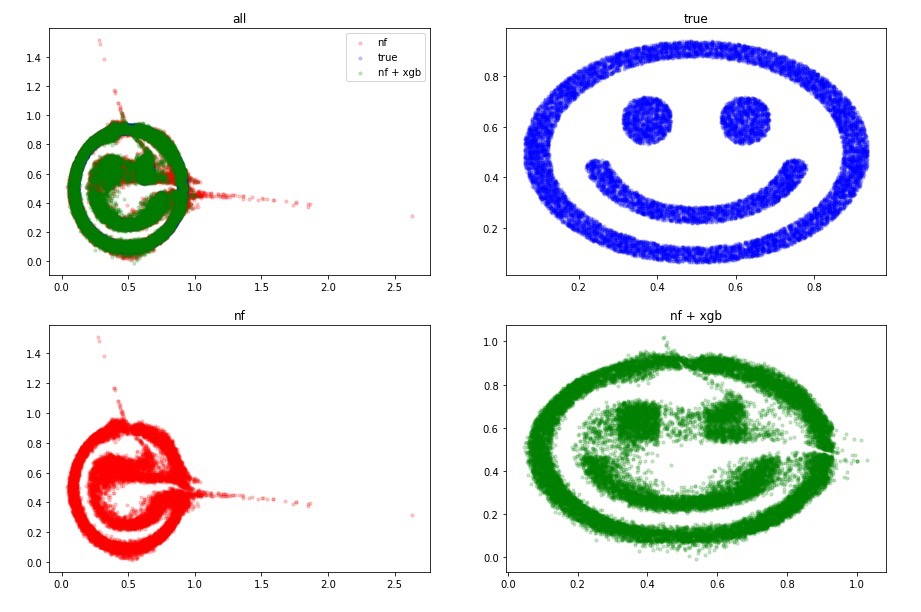
\includegraphics[width=5.5cm]{imgs/smile.jpeg}
    \end{column}%
    \hfill%
    \begin{column}{.48\textwidth}
      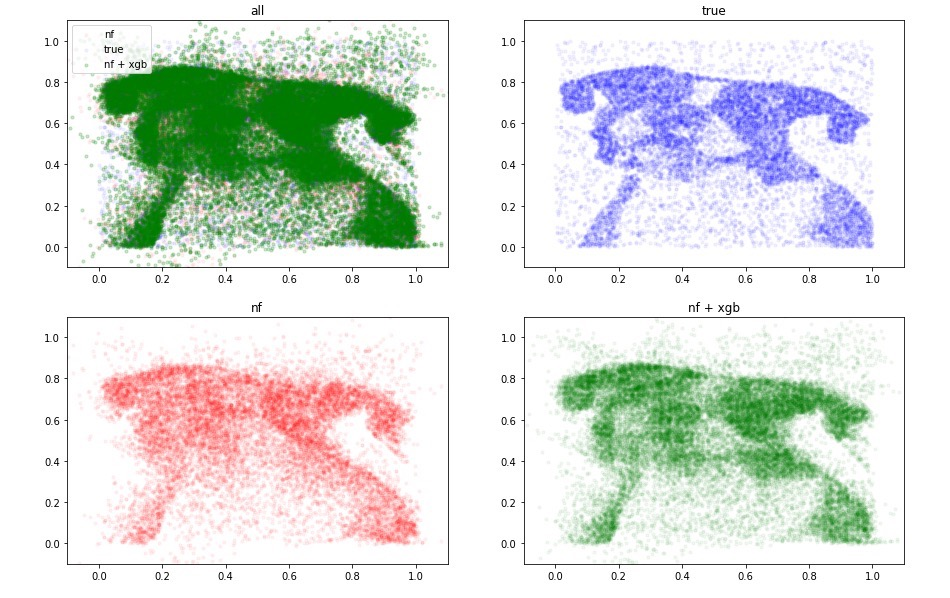
\includegraphics[width=5.5cm]{imgs/dog.jpeg}
    \end{column}%
  \end{columns}
\end{frame}

\begin{frame}{Current results}
  GAS dataset
  \begin{itemize}
    \item SOTA: maf(10) $\to$ 10.08 log likelihood
    \item Ours: maf(5) $\to$ 9.48 log likelihood $\to$ 10.23 ll after calibration by Catboost(2k trees)
  \end{itemize}
\end{frame}

\begin{frame}{Future work}
  \begin{itemize}
    \item KL finetuning nf
    \item Conditional sampling
  \end{itemize}
\end{frame}

\begin{frame}{FAQ}
  \begin{itemize}
    \item What happens if $P = Q$ (perfect nf)? \\
    Then $\forall x ~ clf\_logit(x) = 0$, acceptance rate of rejection sampling = $1$.
    \item What happens if $P$ is trivial (e. g. uniform)? \\
    Then $\exists x ~ clf\_logit(x) \to \infty$, acceptance rate of rejection sampling $\to 0$.
  \end{itemize}
\end{frame}

\begin{frame}
\huge{\centerline{The End}}
\end{frame}

\end{document}
